\mySection{13.2 The $F$ Test for a Randomized Block Design}
%-------------- start slide -------------------------------%{{{
\begin{frame}
	% {\S\: 13.2 The $F$ Test for a Randomized Block Design}

	\begin{enumerate}
		\item[Setup] $Y_{ij}$ indep. $\sim N(\mu_j+\beta_i,\sigma^2)$, i.e., $Y_{ij} = \mu_j+\beta_i+\epsilon_{ij}$, $\epsilon_{ij}$ i.i.d. $\sim N(0,\sigma^2)$
			\vfill
		\item[]
			\begin{center}
				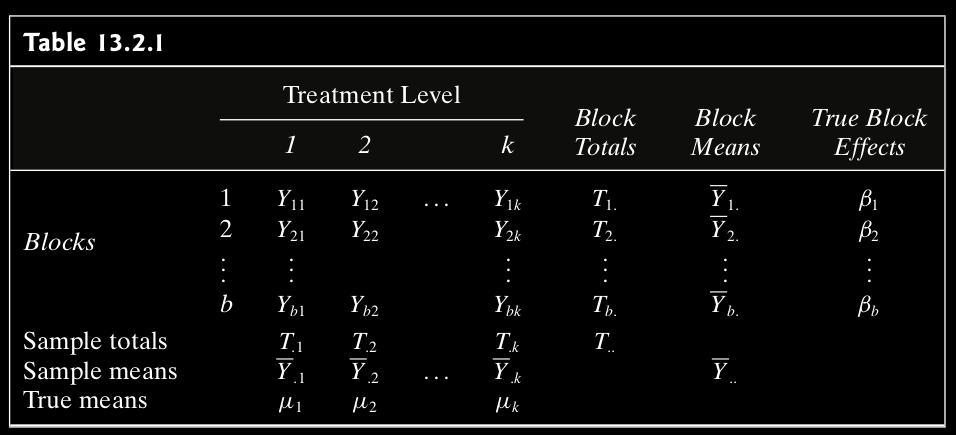
\includegraphics[scale=0.25]{Table_13-2-1-neg.png}
			\end{center}
	\end{enumerate}
\end{frame}
%-------------- end slide -------------------------------%}}}
%-------------- start slide -------------------------------%{{{
\begin{frame}[fragile]
	\begin{enumerate}
		\item[Recall] For one-way ANOVA,
			\[
				Y_{ij} = \textcolor{red}{\mu_j} + \epsilon_{ij}
			\]
		\item[]
			\[\Downarrow\]
		\item[]
	\begin{align*}
		SSTOT = & \sum_{i=1}^b\sum_{j=1}^k \left(Y_{ij}-\overline{Y}_{\cdot\cdot} \right)^2
		     \\ & =  \sum_{i=1}^b\sum_{j=1}^k\left[ \left(Y_{ij}-\textcolor{red}{\overline{Y}_{\cdot j}} \right)+\left(\textcolor{red}{\overline{Y}_{\cdot j}} - \overline{Y}_{\cdot\cdot}\right)\right]^2
		     \\ & =  \sum_{i=1}^b\sum_{j=1}^k\left(Y_{ij}-\overline{Y}_{\cdot j} \right)^2+ \text{zero cross term}+\sum_{i=1}^b\sum_{j=1}^k\left(\overline{Y}_{\cdot j} - \overline{Y}_{\cdot\cdot}\right)^2
		     \\ & =  \sum_{i=1}^b\sum_{j=1}^k\left(Y_{ij}-\overline{Y}_{\cdot j} \right)^2+ \textcolor{red}{b\sum_{j=1}^k \left(\overline{Y}_{\cdot j} - \overline{Y}_{\cdot\cdot}\right)^2
}		      \\&= SSE +\textcolor{red}{SSTR}
	\end{align*}
	\end{enumerate}
\end{frame}
%-------------- end slide -------------------------------%}}}
%-------------- start slide -------------------------------%{{{
\begin{frame}[fragile]
	\begin{center}
		\begin{tabular}{ccccc}
			$\displaystyle SSTOT$ &
			= &
			$\displaystyle SSE$ &
			+ &
			$\displaystyle \textcolor{red}{SSTR}$ \\ \\
			  &$\Downarrow$&&& \\ \\
			$\displaystyle \frac{SSTOT}{\sigma^2}$ &
			= &
			$\displaystyle \frac{SSE}{\sigma^2}$ &
			+ &
			$\displaystyle \frac{\textcolor{red}{SSTR}}{\sigma^2}$ \\ \\
			$\wr$&& $\wr$ &  & $\wr$ \\ \\
			$\chi^2(bk-1)$ && $\chi^2(bk-k)$ & $\perp$ & $\chi^2(k-1)$
			\\[2em]
			Under $H_0$& & \checkmark && Under $H_0$
		\end{tabular}
\vfill
\[
H_0: \mu_1=\cdots =\mu_k
\]
	\end{center}
\end{frame}
%-------------- end slide -------------------------------%}}}
%-------------- start slide -------------------------------%{{{
\begin{frame}[fragile]
	\begin{enumerate}
		\item[Symmetry] If
			\[
				Y_{ij} = \textcolor{cyan}{\beta_i} + \epsilon_{ij}
			\]
		\item[]
			\[\Downarrow\]
		\item[]
	\begin{align*}
		SSTOT = & \sum_{i=1}^b\sum_{j=1}^k \left(Y_{ij}-\overline{Y}_{\cdot\cdot} \right)^2
		     \\ & =  \sum_{i=1}^b\sum_{j=1}^k\left[ \left(Y_{ij}-\textcolor{cyan}{\overline{Y}_{i\cdot}} \right)+\left(\textcolor{cyan}{\overline{Y}_{i\cdot}} - \overline{Y}_{\cdot\cdot}\right)\right]^2
		     \\ & =  \sum_{i=1}^b\sum_{j=1}^k\left(Y_{ij}-\overline{Y}_{i\cdot} \right)^2+ \text{zero cross term}+\sum_{i=1}^b\sum_{j=1}^k\left(\overline{Y}_{i\cdot} - \overline{Y}_{\cdot\cdot}\right)^2
		     \\ & =  \sum_{i=1}^b\sum_{j=1}^k\left(Y_{ij}-\overline{Y}_{i\cdot} \right)^2+ \textcolor{cyan}{k\sum_{i=1}^b\left(\overline{Y}_{i\cdot} - \overline{Y}_{\cdot\cdot}\right)^2
}		      \\&= SSE +\textcolor{cyan}{SSB}
	\end{align*}
	\end{enumerate}
\end{frame}
%-------------- end slide -------------------------------%}}}
%-------------- start slide -------------------------------%{{{
\begin{frame}[fragile]
	\begin{center}
		\begin{tabular}{ccccc}
			$\displaystyle SSTOT$ &
			= &
			$\displaystyle SSE$ &
			+ &
			$\displaystyle \textcolor{cyan}{SSB}$ \\ \\
			  &$\Downarrow$&&& \\ \\
			$\displaystyle \frac{SSTOT}{\sigma^2}$ &
			= &
			$\displaystyle \frac{SSE}{\sigma^2}$ &
			+ &
			$\displaystyle \frac{\textcolor{cyan}{SSB}}{\sigma^2}$ \\ \\
			$\wr$&& $\wr$ &  & $\wr$ \\ \\
			$\chi^2(bk-1)$ && $\chi^2(bk-b)$ & $\perp$ & $\chi^2(b-1)$
			\\[2em]
			Under $\widetilde H_0$& & \checkmark && Under $\widetilde H_0$
		\end{tabular}
		\vfill
		\[
		\widetilde H_0 : \beta_1=\cdots = \beta_b
		\]
	\end{center}
\end{frame}
%-------------- end slide -------------------------------%}}}
%-------------- start slide -------------------------------%{{{
\begin{frame}[fragile]
	\begin{enumerate}
		\item[Similarly] If
			\[
				Y_{ij} = \textcolor{red}{\mu_j} + \textcolor{cyan}{\beta_i} + \epsilon_{ij}
			\]
		\item[]
			\[\Downarrow\]
		\item[]
	\begin{align*}
		\hspace{-4em}SSTOT =  & \sum_{i=1}^b\sum_{j=1}^k \left(Y_{ij}-\overline{Y}_{\cdot\cdot} \right)^2 \\
                          & =  \sum_{i=1}^b\sum_{j=1}^k\left[ \left(Y_{ij}-\textcolor{cyan}{\overline{Y}_{i\cdot}} - \textcolor{red}{\overline{Y}_{\cdot j}}+\overline{Y}_{\cdot\cdot} \right)+\left(\textcolor{cyan}{\overline{Y}_{i\cdot}} - \overline{Y}_{\cdot\cdot}\right)+\left(\textcolor{red}{\overline{Y}_{\cdot j}}- \overline{Y}_{\cdot\cdot}\right)\right]^2 \\
													& =  \sum_{i=1}^b\sum_{j=1}^k\left(Y_{ij}-\overline{Y}_{i\cdot} -\overline{Y}_{\cdot j}+\overline{Y}_{\cdot\cdot}\right)^2 +\sum_{i=1}^b\sum_{j=1}^k\left(\overline{Y}_{i\cdot} - \overline{Y}_{\cdot\cdot}\right)^2 \\
													&\quad+\sum_{i=1}^b\sum_{j=1}^k\left(\overline{Y}_{\cdot j} - \overline{Y}_{\cdot\cdot}\right)^2 + \text{zero cross terms} \\
													& =  \sum_{i=1}^b\sum_{j=1}^k\left(Y_{ij}-\overline{Y}_{i\cdot} -\overline{Y}_{\cdot j} + \overline{Y}_{\cdot\cdot} \right)^2+\textcolor{cyan}{k\sum_{i=1}^b\left(\overline{Y}_{i\cdot} - \overline{Y}_{\cdot\cdot}\right)^2} +\textcolor{red}{b\sum_{j=1}^k\left(\overline{Y}_{\cdot j} - \overline{Y}_{\cdot\cdot}\right)^2} \\
													&= SSE + \textcolor{cyan}{SSB} + \textcolor{red}{SSTR}
	\end{align*}
	\end{enumerate}
\end{frame}
%-------------- end slide -------------------------------%}}}
%-------------- start slide -------------------------------%{{{
\begin{frame}[fragile]
	\begin{center}
		\begin{tabular}{ccccccc}
			$\displaystyle SSTOT$ &
			= &
			$\displaystyle SSE$ &
			+ &
			$\displaystyle \textcolor{cyan}{SSB}$ &+& $\displaystyle \textcolor{red}{SSTR}$ \\ \\
					    &$\Downarrow$&&& &&\\ \\
			$\displaystyle \frac{SSTOT}{\sigma^2}$ &
			= &
			$\displaystyle \frac{SSE}{\sigma^2}$ &
			+ &
			$\displaystyle \frac{\textcolor{cyan}{SSB}}{\sigma^2}$ &+& $\displaystyle \frac{\textcolor{red}{SSTR}}{\sigma^2}$ \\ \\
			$\wr$&& $\wr$ &  & $\wr$ && $\wr$ \\ \\
			$\chi^2(bk-1)$ && $\chi^2((k-1)(b-1))$ & $\perp$ & $\chi^2(b-1)$ & $\perp$ & $\chi^2(k-1)$
			\\[2em]
			Under $H_0$ or $\widetilde H_0$& &\checkmark&& under $\widetilde{H}_0$ && under $H_0$
		\end{tabular}
		\vfill
		\[
		\widetilde H_0 : \beta_1=\cdots = \beta_b
		\qquad\text{and}\qquad
		H_0: \mu_1\cdots = \mu_k
		\]
	\end{center}
\end{frame}
%-------------- end slide -------------------------------%}}}
%-------------- start slide -------------------------------%{{{
\begin{frame}[fragile]


	\phantom{a}\hfill\begin{minipage}{0.6\textwidth}
		\[
		H_0: \mu_1\cdots = \mu_k
		\]
		\[
		\Downarrow
		\]
	\end{minipage}

% \vfill
	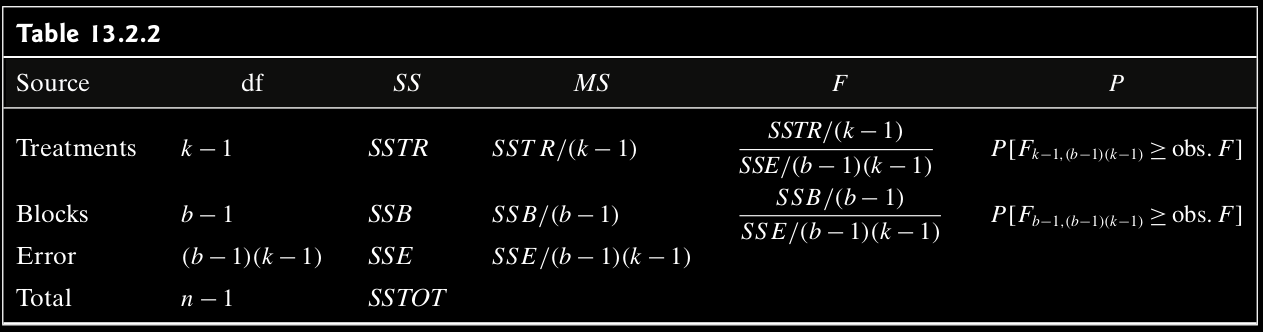
\includegraphics[scale=0.25]{Table_13-2-2-neg.png}
% \vfill

	\phantom{a}\hfill\begin{minipage}{0.6\textwidth}
		\[
		\Uparrow
		\]
	\[
		\widetilde H_0 : \beta_1=\cdots = \beta_b
	\]
	\end{minipage}
\end{frame}
%-------------- end slide -------------------------------%}}}
%-------------- start slide -------------------------------%{{{
\begin{frame}[fragile]{Computing formulas}
\[
	C =  \frac{T_{\cdot\cdot}^2}{bk}
\]
\vfill
\[
	\textcolor{red}{SSTR} = b\sum_{j=1}^k\left(\overline{Y}_{\cdot j}-\overline{Y}_{\cdot\cdot}\right)^2
	= b\sum_{j=1}^k \overline{Y}_{\cdot j}^2 - bk \overline{Y}_{\cdot\cdot}^2 =
	\frac{1}{b}\sum_{j=1}^k \overline{T}_{\cdot j}^2 -C.
\]
\vfill
\[
	\textcolor{cyan}{SSB} = k\sum_{i=1}^b\left(\overline{Y}_{i\cdot}-\overline{Y}_{\cdot\cdot}\right)^2
	= k\sum_{i=1}^b \overline{Y}_{i\cdot}^2 - bk \overline{Y}_{\cdot\cdot}^2 =
	\frac{1}{k}\sum_{j=1}^k \overline{T}_{i\cdot}^2 -C.
\]
\vfill
\[
	SSTOT =
	\sum_{i=1}^b\sum_{j=1}^k \left(Y_{ij}-\overline{Y}_{\cdot\cdot}\right)^2
	=\sum_{i=1}^b\sum_{j=1}^k Y_{ij}^2-bk\overline{Y}_{\cdot\cdot}^2
	=\sum_{i=1}^b\sum_{j=1}^k Y_{ij}^2-C.
\]
\vfill
\[
SSE = SSTOT-\textcolor{cyan}{SSTR}-\textcolor{red}{SSB}
\]
\end{frame}
%-------------- end slide -------------------------------%}}}
%-------------- start slide -------------------------------%{{{
\begin{frame}[fragile]

\begin{enumerate}
	\item[E.g.] Two methods to test wines: whether these two procedures produce the same measurements?
		\vfill
	\item[]
		\begin{center}
			\begin{tabular}{l|cc}
				& DRS-FTIR & Standard \\
				\hline
				White wine 1 & 112.9 & 115.1  \\
				White wine 2 & 123.1 & 125.6  \\
				Red wine 1 &   135.2 & 132.4  \\
				Red wine 2 &   140.2 & 143.7
				\\
\hline
			\end{tabular}
			\\
			\vfill
			Test at $\alpha=0.05$
			\[
				H_0: \mu_{DRS} = \mu_{STD}\quad\text{v.s.}\quad H_1: \mu_{DRS} \ne \mu_{STD}
			\]
and
			\[
				\widetilde H_0: \mu_{W1} = \mu_{W2}=\mu_{R1} = \mu_{R2}\quad\text{v.s.}\quad \widetilde H_1: \text{not equal}
			\]
		\end{center}
\end{enumerate}

\end{frame}
%-------------- end slide -------------------------------%}}}
%-------------- start slide -------------------------------%{{{
\begin{frame}[fragile]
	\begin{center}
	\begin{minipage}{0.48\textwidth}
	\begin{lstlisting}
> # Case Study 13.2.1
> # install.packages("ggpubr")
> DIRS <- c(112.9, 123.1, 135.2, 140.2)
> STD <- c(115.1, 125.6, 132.4, 143.7)
> Wines <- c("W1", "W2", "R1", "R2")
> # Create a data frame
> my_data <- data.frame(
+   method = rep(c("DIRS", "STD"), each =4),
+   types = c(Wines,Wines),
+   concentration = c(DIRS,  STD)
+ )
> # Show data
> print(my_data)
  method types concentration
1   DIRS    W1         112.9
2   DIRS    W2         123.1
3   DIRS    R1         135.2
4   DIRS    R2         140.2
5    STD    W1         115.1
6    STD    W2         125.6
7    STD    R1         132.4
8    STD    R2         143.7
	\end{lstlisting}
	\end{minipage}
	\end{center}
\end{frame}
%-------------- end slide -------------------------------%}}}
%-------------- start slide -------------------------------%{{{
\begin{frame}[fragile]
\small
	\begin{minipage}{0.48\textwidth}
	\begin{lstlisting}
> # Compute t-test with equal variances
> res <- t.test(concentration ~ method,
+               data = my_data,
+               var.equal = TRUE)
> res

	Two Sample t-test

data:  concentration by method
t = -0.15721, df = 6, p-value = 0.8802
alternative hypothesis: true difference in means is not equal to 0
95 percent confidence interval:
 -22.362  19.662
sample estimates:
mean in group DIRS  mean in group STD
            127.85             129.20
	\end{lstlisting}
	\end{minipage}
	\hfill
	\begin{minipage}{0.5\textwidth}
	\begin{lstlisting}
> # Compute t-test with unequal variances
> res <- t.test(concentration ~ method,
+               data = my_data,
+               var.equal = FALSE)
> res

	Welch Two Sample t-test

data:  concentration by method
t = -0.15721, df = 5.9968, p-value = 0.8802
alternative hypothesis: true difference in means is not equal to 0
95 percent confidence interval:
 -22.3647  19.6647
sample estimates:
mean in group DIRS  mean in group STD
            127.85             129.20
	\end{lstlisting}
	\end{minipage}
	\vspace{-3em}

\begin{minipage}{0.47\textwidth}
	\begin{lstlisting}
> # The following one-way ANOVA is equivalent
> # to the two-sample t test
> library(car)
> model3 = lm(concentration ~ method,
+             data=my_data)
> Anova(model3)
Anova Table (Type II tests)

Response: concentration
          Sum Sq Df F value Pr(>F)
method      3.64  1  0.0247 0.8802
Residuals 884.87  6
	\end{lstlisting}
		\end{minipage}
\hfill
\begin{minipage}{0.4\textwidth}
\vspace{-1em}
	\begin{enumerate}
		\item Classical method
		\item Welch approximation
		\item one-way ANOVA
			\[\Downarrow\]
			\begin{center}The same answer \\($p$-value)
			\end{center}
		\item[Concl.] Fail to reject $H_0$
	\end{enumerate}
\end{minipage}
\end{frame}
%-------------- end slide -------------------------------%}}}
%-------------- start slide -------------------------------%{{{
\begin{frame}[fragile]
	\begin{center}
		\begin{minipage}{0.47\textwidth}
	\begin{lstlisting}
> # Now let's carry out two-way ANOVA
> library(car)
> model = lm(concentration ~ method + types,
+            data=my_data)
> Anova(model)
Anova Table (Type II tests)

Response: concentration
          Sum Sq Df F value   Pr(>F)
method      3.65  1  0.9154 0.409258
types     872.92  3 73.0787 0.002652 **
Residuals  11.94  3
	\end{lstlisting}
		\end{minipage}
		% \vfill
		\hfill
		\begin{minipage}{0.48\textwidth}
	\begin{lstlisting}
> # Now let's try one-way ANOVA
> model2 = lm(concentration ~ types,
+             data=my_data)
> Anova(model2)
Anova Table (Type II tests)

Response: concentration
          Sum Sq Df F value    Pr(>F)
types     872.92  3  74.657 0.0005739 ***
Residuals  15.59  4
---
Signif. codes:  0 '***' 0.001 '**' 0.01 '*' 0.05 '.' 0.1 ' ' 1
	\end{lstlisting}
		\end{minipage}
	\end{center}

\vfill
	\begin{enumerate}
		\item Fail to reject $H_0$
		\item Reject $\widetilde H_0$
	\end{enumerate}
\end{frame}
%-------------- end slide -------------------------------%}}}
%-------------- start slide -------------------------------%{{{
\begin{frame}[fragile]

	\begin{enumerate}
		\item[E.g. 2]{\url{https://rcompanion.org/rcompanion/d_08.html}}
			\begin{center}
				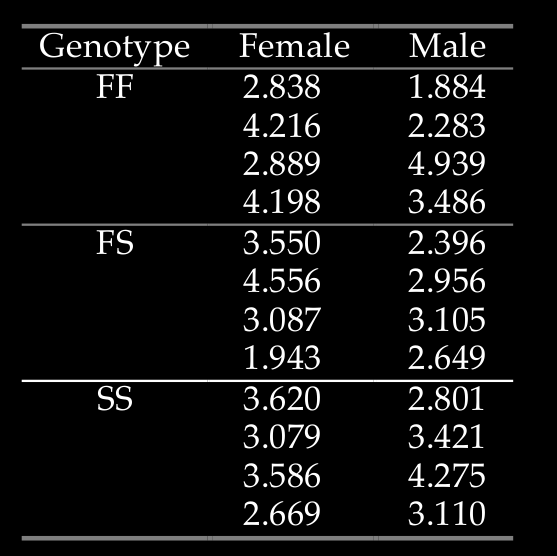
\includegraphics[scale=0.25]{Two-Way-Anova-Data1-neg.png}
				\vfill
				Test at $\alpha=0.05$\\
				\[
				H_0: \mu_F = \mu_M \quad v.s.\quad
				H_1: \mu_F\ne \mu_F
				\]
				and
				\[
					\widetilde H_0: \mu_{FF} = \mu_{S}= \mu_{SS} \quad v.s. \quad \widetilde H_1: \text{not all equal}
				\]
			\end{center}
	\end{enumerate}
\end{frame}
%-------------- end slide -------------------------------%}}}
%-------------- start slide -------------------------------%{{{
\begin{frame}[fragile]
	\begin{minipage}{0.45\textwidth}
	\begin{lstlisting}
> Data
   id    Sex Genotype Activity
1   1   male       ff    1.884
2   2   male       ff    2.283
3   3   male       fs    2.396
4   4 female       ff    2.838
5   5   male       fs    2.956
6   6 female       ff    4.216
7   7 female       ss    3.620
8   8 female       ff    2.889
9   9 female       fs    3.550
10 10   male       fs    3.105
11 11 female       fs    4.556
12 12 female       fs    3.087
13 13   male       ff    4.939
14 14   male       ff    3.486
15 15 female       ss    3.079
16 16   male       fs    2.649
	\end{lstlisting}
	\end{minipage}
	\hfill
	\begin{minipage}{0.45\textwidth}
	\begin{lstlisting}
17 17 female       fs    1.943
18 19 female       ff    4.198
19 20 female       ff    2.473
20 22 female       ff    2.033
21 24 female       fs    2.200
22 25 female       fs    2.157
23 26   male       ss    2.801
24 28   male       ss    3.421
25 29 female       ff    1.811
26 30 female       fs    4.281
27 32 female       fs    4.772
28 34 female       ss    3.586
29 36 female       ff    3.944
30 38 female       ss    2.669
31 39 female       ss    3.050
32 41   male       ss    4.275
33 43 female       ss    2.963
34 46 female       ss    3.236
35 48 female       ss    3.673
36 49   male       ss    3.110
	\end{lstlisting}
	\end{minipage}
\end{frame}
%-------------- end slide -------------------------------%}}}
%-------------- start slide -------------------------------%{{{
\begin{frame}[fragile]
	\begin{minipage}{0.46\textwidth}
	\begin{lstlisting}
> # Two-way ANOVA
> model = lm(Activity ~ Sex + Genotype,
+            data=Data)
> Anova(model, type="II")
Anova Table (Type II tests)

Response: Activity
           Sum Sq Df F value Pr(>F)
Sex        0.0681  1  0.0888 0.7676
Genotype   0.2772  2  0.1808 0.8354
Residuals 24.5285 32
> # One-way ANOVA
> model_Sex = lm(Activity ~ Sex,
+                data=Data)
> Anova(model_Sex, type="II")
Anova Table (Type II tests)

Response: Activity
           Sum Sq Df F value Pr(>F)
Sex        0.0681  1  0.0933 0.7619
Residuals 24.8057 34
> # One-way ANOVA
> model_Genotype = lm(Activity ~ Genotype,
+                data=Data)
> Anova(model_Genotype, type="II")
Anova Table (Type II tests)

Response: Activity
           Sum Sq Df F value Pr(>F)
Genotype   0.2772  2   0.186 0.8312
Residuals 24.5965 33
	\end{lstlisting}
	\end{minipage}
\end{frame}
%-------------- end slide -------------------------------%}}}
%-------------- start slide -------------------------------%{{{
\begin{frame}[fragile]{Tuckey's pairwise comparison}

	\[
		\text{Replace} \quad Q_{\alpha, k,b(k-k)} \quad \text{by}\quad
		Q_{\alpha, k,(b-1)(k-1)}
	\]
	\vfill
	\begin{minipage}{0.47\textwidth}
	\begin{lstlisting}
> # Tukey's pairwise comparison (One-way)
> model1 = aov(Activity ~ Genotype,
+                       data=Data)
> TukeyHSD(model1, "Genotype", ordered = TRUE)
  Tukey multiple comparisons of means
    95% family-wise confidence level
    factor levels have been ordered

Fit: aov(formula = Activity ~ Genotype, data = Data)

$Genotype
            diff        lwr      upr     p adj
fs-ff 0.05483333 -0.8100204 0.919687 0.9867505
ss-ff 0.20741667 -0.6574370 1.072270 0.8272105
ss-fs 0.15258333 -0.7122704 1.017437 0.9021607
	\end{lstlisting}
	\end{minipage}
	\hfill
	\begin{minipage}{0.47\textwidth}
	\begin{lstlisting}
> # Tukey's pairwise comparison (Two-way)
> model2 = aov(Activity ~ Sex + Genotype,
+            data=Data)
> TukeyHSD(model2, "Genotype", ordered = TRUE)
  Tukey multiple comparisons of means
    95% family-wise confidence level
    factor levels have been ordered

Fit: aov(formula = Activity ~ Sex + Genotype, data = Data)

$Genotype
            diff        lwr       upr    p adj
fs-ff 0.05483333 -0.8234920 0.9331586 0.987114
ss-ff 0.20741667 -0.6709086 1.0857420 0.831554
ss-fs 0.15258333 -0.7257420 1.0309086 0.904729
	\end{lstlisting}
	\end{minipage}
\end{frame}
%-------------- end slide -------------------------------%}}}
%-------------- start slide -------------------------------%{{{
\begin{frame}[fragile]

	\begin{enumerate}
		\item[Remark] By two-way ANOVA, or through blocking one factor, we obtain
			\vfill
		\item larger $p$-values:
		\item[] more conservative to reject $H_0$.
			\vfill
		\item wider C.I.'s:
		\item[] more conservative on our estimates.
	\end{enumerate}
\end{frame}
%-------------- end slide -------------------------------%}}}
